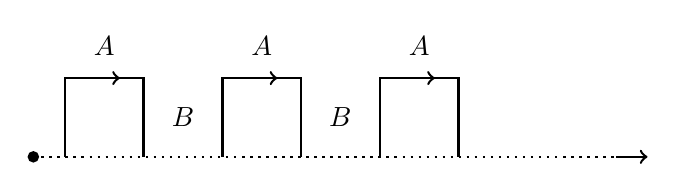
\begin{tikzpicture}[line width=0.9pt]
  % baseline (dotted), with a dot on far left and arrow at far right
  \draw[dotted] (-0.4,0) -- (7.0,0);
  \filldraw (-0.4,0) circle (1.6pt);
  \draw[->] (7.0,0) -- (7.4,0);
  % square-wave step profile with three "A" plateaus and two "B" gaps, each 2 units wide, height 1
  \foreach \x in {0,2,4} {
    \draw (\x,0) -- (\x,1) -- (\x+1,1) -- (\x+1,0);
    \draw[->] (\x+0.3,1) -- (\x+0.7,1);
    \node[above] at (\x+0.5,1.15) {$A$};
  }
  \node at (1.5,0.5) {$B$};
  \node at (3.5,0.5) {$B$};
\end{tikzpicture}
